\documentclass[aspectratio=169,10pt]{beamer}

\usetheme{Madrid}
\usecolortheme{seahorse}
\usepackage{amsmath, amssymb, amsfonts}
\usepackage{listings}
\usepackage{xcolor}
\usepackage{graphicx}
\usepackage{booktabs}
\usepackage{hyperref}
\usepackage{tikz}
\usetikzlibrary{shapes, arrows, decorations.pathreplacing}

% Set graphics path
\graphicspath{{figures/}}

% Code listing style
\lstset{
    basicstyle=\ttfamily\small,
    commentstyle=\color{green!50!black}\itshape,
    keywordstyle=\color{blue}\bfseries,
    stringstyle=\color{red},
    breaklines=true,
    frame=single,
    numbers=left,
    numberstyle=\tiny\color{gray},
    showstringspaces=false,
    language=Python
}

% Footer
\setbeamertemplate{footline}[frame number]

% Title
\title{Linear Operators: Basic Theory}
\subtitle{Pathak -- Nonlinear Analysis and Fixed Point Theory (2018)}
\author{Lecture Slides}
\date{\today}

\begin{document}

% Title slide
\begin{frame}
    \titlepage
    \vspace{-1cm}
    {\small Chapter 5d: Bounded Linear Operators and Operator Spaces}
\end{frame}

% Table of Contents
\begin{frame}{Outline}
    \tableofcontents
\end{frame}

\section{Introduction to Linear Operators}

\begin{frame}{What is an Operator?}
    \begin{definition}
        An \textbf{operator} $A : X \to Y$ maps vectors from one space $X$ (domain) to another space $Y$ (codomain).
    \end{definition}

    \vspace{0.5cm}

    \begin{block}{Key Concept}
        An operator is a generalization of the concept of a function to vector spaces. It can be thought of as an object that ``acts on'' vectors to transform them.
    \end{block}

    \vspace{0.5cm}

    \textbf{Domains of application:}
    \begin{itemize}
        \item Matrix equations: $A : \mathbb{R}^n \to \mathbb{R}^m$
        \item Integral transforms: $A : L^2[a,b] \to L^2[a,b]$
        \item Differential equations: $A : C[a,b] \to C[a,b]$
        \item Functional analysis: $A : X \to Y$ for Banach spaces $X, Y$
    \end{itemize}
\end{frame}

\begin{frame}{Linear Operators}
    \begin{definition}
        Let $X$ and $Y$ be vector spaces over the same field $\mathbb{K}$ (where $\mathbb{K} = \mathbb{R}$ or $\mathbb{C}$), and let $A : X \to Y$ be an operator with domain $D(A)$ and range $R(A)$. Then $A$ is a \textbf{linear operator} if:

        \begin{enumerate}
            \item \textbf{Additivity}: $A(x + y) = Ax + Ay$ for all $x, y \in X$
            \item \textbf{Homogeneity}: $A(\alpha x) = \alpha A(x)$ for all $x \in X$, $\alpha \in \mathbb{K}$
        \end{enumerate}
    \end{definition}

    \vspace{0.3cm}

    \begin{block}{Equivalent Formulation}
        $A$ is linear if and only if
        $$A(\alpha x + \beta y) = \alpha A(x) + \beta A(y)$$
        for all $x, y \in X$ and $\alpha, \beta \in \mathbb{K}$.
    \end{block}

    \vspace{0.3cm}

    If $Y = \mathbb{R}$ (or $\mathbb{C}$), then $A$ is called a \textbf{linear functional}.
\end{frame}

\begin{frame}[fragile]{Examples of Linear Operators}
    \begin{example}[Dot Product on $\mathbb{R}^n$]
        Let $X = \mathbb{R}^n$, $Y = \mathbb{R}$, and $A : \mathbb{R}^n \to \mathbb{R}$ defined by:
        $$Ax = \sum_{i=1}^{n} a_i x_i \quad \text{(linear functional)}$$
    \end{example}

    \begin{example}[Shift Operator on $\ell^2$]
        Let $X = Y = \ell^2$ (square-summable sequences). Define:
        $$Ax = \left(x_1, \frac{x_2}{2}, \frac{x_3}{3}, \ldots, \frac{x_n}{n}, \ldots\right)$$
        Check: $A(\alpha x + \beta y) = \alpha Ax + \beta Ay$ \checkmark
    \end{example}

    \begin{example}[Integration on $L^2[0, 2\pi]$]
        Let $X = L^2[0, 2\pi]$, $Y = \mathbb{R}$, and
        $$Ax = \int_0^{2\pi} x(t)y(t) \, dt$$
        where $y$ is a fixed function in $L^2[0, 2\pi]$.
    \end{example}
\end{frame}

\begin{frame}{Properties of Linear Operators}
    \begin{theorem}[Proposition 1.7]
        Let $X$ and $Y$ be linear spaces and $A : X \to Y$ a linear operator. Then:
    \end{theorem}

    \begin{enumerate}
        \item $A(0) = 0$ (maps zero element to zero)

        \item The range $R(A) = \{y \in Y : y = Ax \text{ for some } x \in X\}$ is a linear subspace of $Y$

        \item $A$ is one-to-one (injective) if and only if $Ax = 0 \implies x = 0$

        \item If $A : X \to Y$ is one-to-one, then $A^{-1}$ exists on $R(A)$ and is linear

        \item If $\dim(X) = n < \infty$ and $A^{-1}$ exists, then $\dim(R(A)) = n$
    \end{enumerate}
\end{frame}

\section{Bounded Linear Operators}

\begin{frame}{Continuity and Linearity}
    \begin{theorem}[Theorem 1.12]
        Let $X$ and $Y$ be normed spaces and $A : X \to Y$ a linear operator. If $A$ is continuous at a single point in $X$, then $A$ is continuous throughout space $X$.
    \end{theorem}

    \vspace{0.5cm}

    \begin{proof}[Proof Sketch]
        Suppose $A$ is continuous at $x_0$ and $x_n \to x$. Then:
        \begin{align*}
            \|Ax_n - Ax\| &= \|A(x_n - x + x_0) - Ax_0\| \\
            &\to 0 \quad \text{(as $x_n \to x$)}
        \end{align*}
        Thus $A$ is continuous at every point $x \in X$.
    \end{proof}
\end{frame}

\begin{frame}{Definition of Bounded Linear Operator}
    \begin{definition}
        Let $X$ and $Y$ be normed spaces and $A : X \to Y$ a linear operator. Then $A$ is \textbf{bounded} if there exists a constant $M > 0$ such that
        $$\|Ax\| \leq M\|x\| \quad \text{for all } x \in X.$$
    \end{definition}

    \vspace{0.5cm}

    \begin{block}{Important Distinction}
        A bounded operator does NOT map the entire space $X$ into a bounded set in $Y$. Rather:
        \begin{itemize}
            \item A bounded operator maps \textbf{bounded sets} to \textbf{bounded sets}
            \item The converse is also true: bounded sets $\to$ bounded sets $\Rightarrow$ bounded operator
        \end{itemize}
    \end{block}

    \vspace{0.3cm}

    \begin{block}{Linear Functional}
        A linear functional $f : X \to \mathbb{R}$ is bounded if
        $$|f(x)| \leq M\|x\| \quad \text{for all } x \in X.$$
    \end{block}
\end{frame}

\begin{frame}[fragile]{Example: Unbounded Linear Operator}
    \begin{example}[Unbounded Functional on $c_{00}$]
        Let $c_{00}$ be the space of finitely nonzero real sequences with supremum norm $\|\cdot\|_\infty$. Define $A : c_{00} \to \mathbb{R}$ by:
        $$Ax = \sum_{i=1}^{n} i \cdot x_i$$
        for $x = (x_1, x_2, \ldots, x_n, 0, 0, \ldots)$.
    \end{example}

    \vspace{0.3cm}

    \textbf{Why is it unbounded?}
    \begin{itemize}
        \item Let $x_n = (0, 0, \ldots, 0, 1/n, 0, \ldots)$ with the 1 in position $n$
        \item Then $\|x_n\|_\infty = 1/n \to 0$
        \item But $A(x_n) = n \cdot (1/n) = 1 \not\to 0$
        \item So the operator is \textbf{discontinuous} at 0, hence unbounded
    \end{itemize}
\end{frame}

\begin{frame}{Bounded $\Leftrightarrow$ Continuous for Linear Operators}
    \begin{theorem}[Theorem 1.13 -- Central Result]
        Let $X$ and $Y$ be normed spaces and $A : X \to Y$ a linear operator. Then $A$ is bounded if and only if it is continuous.
    \end{theorem}

    \vspace{0.5cm}

    \begin{columns}[T]
        \column{0.48\textwidth}
        \textbf{Bounded} $\Rightarrow$ \textbf{Continuous}
        \begin{itemize}
            \item If $\|Ax\| \leq M\|x\|$ for all $x$
            \item Then $x_n \to 0 \implies$
            \item $\|Ax_n\| \leq M\|x_n\| \to 0$
            \item So $A$ is continuous at 0
            \item By Thm 1.12: continuous everywhere
        \end{itemize}

        \column{0.48\textwidth}
        \textbf{Continuous} $\Rightarrow$ \textbf{Bounded}
        \begin{itemize}
            \item Proof by contrapositive
            \item If unbounded: $\|Ax_n\| > n\|x_n\|$ for some sequence
            \item Set $y_n = x_n/(n\|x_n\|)$
            \item Then $y_n \to 0$ but $\|Ay_n\| > 1$
            \item So $A$ is discontinuous at 0
        \end{itemize}
    \end{columns}

    \vspace{0.5cm}

    \begin{alertblock}{Key Insight}
        For linear operators, boundedness and continuity are equivalent! This is a \textbf{fundamental theorem} in functional analysis.
    \end{alertblock}
\end{frame}

\begin{frame}{Operator Norm}
    \begin{definition}
        For $A \in B(X,Y)$ (space of bounded linear operators), the \textbf{operator norm} is:
        $$\|A\|_B = \inf\{M : \|Ax\| \leq M\|x\|, \forall x \in X\}$$
    \end{definition}

    \vspace{0.3cm}

    \begin{block}{Equivalent Formulations}
        All of the following are equivalent:
        \begin{align*}
            \|A\|_B &= \sup\left\{\frac{\|Ax\|}{\|x\|} : x \neq 0, x \in X\right\} \\
            &= \sup\{\|Ax\| : \|x\| \leq 1, x \in X\} \\
            &= \sup\{\|Ax\| : \|x\| = 1, x \in X\}
        \end{align*}
    \end{block}

    \vspace{0.3cm}

    \begin{example}[Matrix Operator Norm]
        For $A : \mathbb{R}^n \to \mathbb{R}^m$ (a matrix), $\|A\|_B$ equals the largest singular value of $A$.
    \end{example}
\end{frame}

\begin{frame}{Properties of the Operator Norm}
    \begin{theorem}
        The operator norm on $B(X,Y)$ satisfies:
    \end{theorem}

    \begin{enumerate}
        \item \textbf{Norm property}: $\|Ax\| \leq \|A\|_B \cdot \|x\|$ for all $x \in X$

        \item \textbf{Triangle inequality}: $\|A + B\|_B \leq \|A\|_B + \|B\|_B$

        \item \textbf{Homogeneity}: $\|\lambda A\|_B = |\lambda| \cdot \|A\|_B$ for scalar $\lambda$

        \item \textbf{Composition}: $\|A \circ B\|_B \leq \|A\|_B \cdot \|B\|_B$

        \item \textbf{Identity operator}: $\|I\|_B = 1$ where $I$ is the identity
    \end{enumerate}

    \vspace{0.5cm}

    \begin{block}{Banach Space Structure}
        With the operator norm, $B(X,Y)$ becomes a normed space. It is a \textbf{Banach space} if $Y$ is a Banach space.
    \end{block}
\end{frame}

\section{Spaces of Bounded Linear Operators}

\begin{frame}{The Space $B(X, Y)$}
    \begin{definition}
        Let $X$ and $Y$ be normed spaces. The space $B(X, Y)$ consists of all bounded linear operators from $X$ into $Y$.
    \end{definition}

    \vspace{0.3cm}

    $B(X, Y)$ is a \textbf{linear space} with operations:
    \begin{itemize}
        \item \textbf{Addition}: $(A_1 + A_2)(x) = A_1x + A_2x$
        \item \textbf{Scalar multiplication}: $(\lambda A)(x) = \lambda A(x)$
    \end{itemize}

    \vspace{0.3cm}

    \begin{block}{Banach Space Property}
        If $Y$ is a Banach space, then $B(X, Y)$ is also a \textbf{Banach space} with the operator norm.
    \end{block}

    \vspace{0.3cm}

    \begin{examples}
        \begin{itemize}
            \item $B(\mathbb{R}^n, \mathbb{R}^m)$: all $m \times n$ real matrices
            \item $B(C[a,b], C[a,b])$: multiplication by continuous functions bounded by their maximum
            \item $B(L^2(\Omega), L^2(\Omega))$: integral operators with finite norm
            \item $B(H, H)$ for Hilbert space $H$: all bounded linear functionals
        \end{itemize}
    \end{examples}
\end{frame}

\begin{frame}{Uniform Boundedness Principle}
    \begin{theorem}[Theorem 1.14]
        Let $X$ be a Banach space, $Y$ a normed space, and $\{A_i\}_{i \in I}$ a family of bounded linear operators from $X$ into $Y$ such that $\{A_i x : i \in I\}$ is bounded for each $x \in X$.
    \end{theorem}

    Then $\{A_i\}_{i \in I}$ is a bounded family, i.e., the operators are \textbf{uniformly bounded}:
    $$\sup_{i \in I} \|A_i\|_B < \infty$$

    \vspace{0.5cm}

    \begin{block}{Intuition}
        If a family of operators is \textit{pointwise bounded} (bounded at every point), then it is \textit{uniformly bounded} (bounded with a single constant for all operators).
    \end{block}

    \vspace{0.3cm}

    \begin{alertblock}{Importance}
        This is a \textbf{fundamental principle} in functional analysis with crucial applications to convergence of operator sequences and iterative methods.
    \end{alertblock}
\end{frame}

\begin{frame}{Pointwise Limit of Operator Sequences}
    \begin{theorem}[Theorem 1.15]
        Let $X$ and $Y$ be Banach spaces and $\{A_n\}$ a sequence of bounded operators from $X$ into $Y$. If for each $x \in X$, the sequence $\{A_n x\}$ converges to $Ax$ in $Y$, then:
    \end{theorem}

    \begin{enumerate}
        \item $A$ is a bounded linear operator, i.e., $A \in B(X, Y)$
        \item $\|A\|_B \leq \liminf_{n \to \infty} \|A_n\|_B$
    \end{enumerate}

    \vspace{0.5cm}

    \begin{proof}[Proof Outline]
        \begin{enumerate}
            \item Linearity of $A$ follows from linearity of $A_n$ and continuity of limits
            \item Boundedness of $\{A_n x\}$ for each $x$ combined with Uniform Boundedness Principle gives uniform boundedness
            \item Thus $\|A_n\|_B \leq M$ for all $n$, proving $A$ is bounded
        \end{enumerate}
    \end{proof}
\end{frame}

\section{Convergence in Operator Spaces}

\begin{frame}{Types of Convergence for Operator Sequences}
    \begin{definition}
        Let $\{T_n\}$ be a sequence in $B(X, Y)$ where $(X, \|\cdot\|_X)$ and $(Y, \|\cdot\|_Y)$ are normed spaces:
    \end{definition}

    \begin{enumerate}
        \item \textbf{Uniform convergence}: $\|T_n - T\|_B \to 0$ as $n \to \infty$

        \vspace{0.2cm}

        \item \textbf{Strong convergence}: $\|T_n x - T x\|_Y \to 0$ as $n \to \infty$ for all $x \in X$

        \vspace{0.2cm}

        \item \textbf{Weak convergence}: $|f(T_n x) - f(T x)| \to 0$ as $n \to \infty$ for all $x \in X$ and $f \in Y^*$

        (where $Y^*$ is the dual space of bounded linear functionals on $Y$)
    \end{enumerate}
\end{frame}

\begin{frame}{Hierarchy of Convergence}
    \begin{theorem}
        The following implications hold for operator sequences in $B(X, Y)$:
    \end{theorem}

    \vspace{0.5cm}

    $$\text{Uniform Convergence} \Rightarrow \text{Strong Convergence} \Rightarrow \text{Weak Convergence}$$

    \vspace{0.5cm}

    \begin{columns}[T]
        \column{0.32\textwidth}
        \textbf{Uniform} $\Rightarrow$ \textbf{Strong}
        \begin{small}
            If $\|T_n - T\|_B \to 0$, then:
            \[\begin{aligned}
            \|T_n x - T x\| &\leq \|T_n - T\|_B \|x\| \\
            &\to 0 \, \forall x
            \end{aligned}\]
        \end{small}

        \column{0.32\textwidth}
        \textbf{Strong} $\Rightarrow$ \textbf{Weak}
        \begin{small}
            If $T_n x \to T x$, then:
            \[\begin{aligned}
            |f(T_n x - T x)| &\leq \|f\| \|T_n x - T x\| \\
            &\to 0 \, \forall x, f
            \end{aligned}\]
        \end{small}

        \column{0.32\textwidth}
        \textbf{No reverse implication}
        \begin{small}
            Weak convergence does NOT imply strong, and strong does NOT imply uniform.

            These are proper inclusions.
        \end{small}
    \end{columns}

    \vspace{0.5cm}

    \begin{alertblock}{Convergence Speed}
        Uniform is fastest, weak is slowest. The choice depends on the application and available regularity.
    \end{alertblock}
\end{frame}

\begin{frame}{Convergence Visualization}
    \begin{center}
        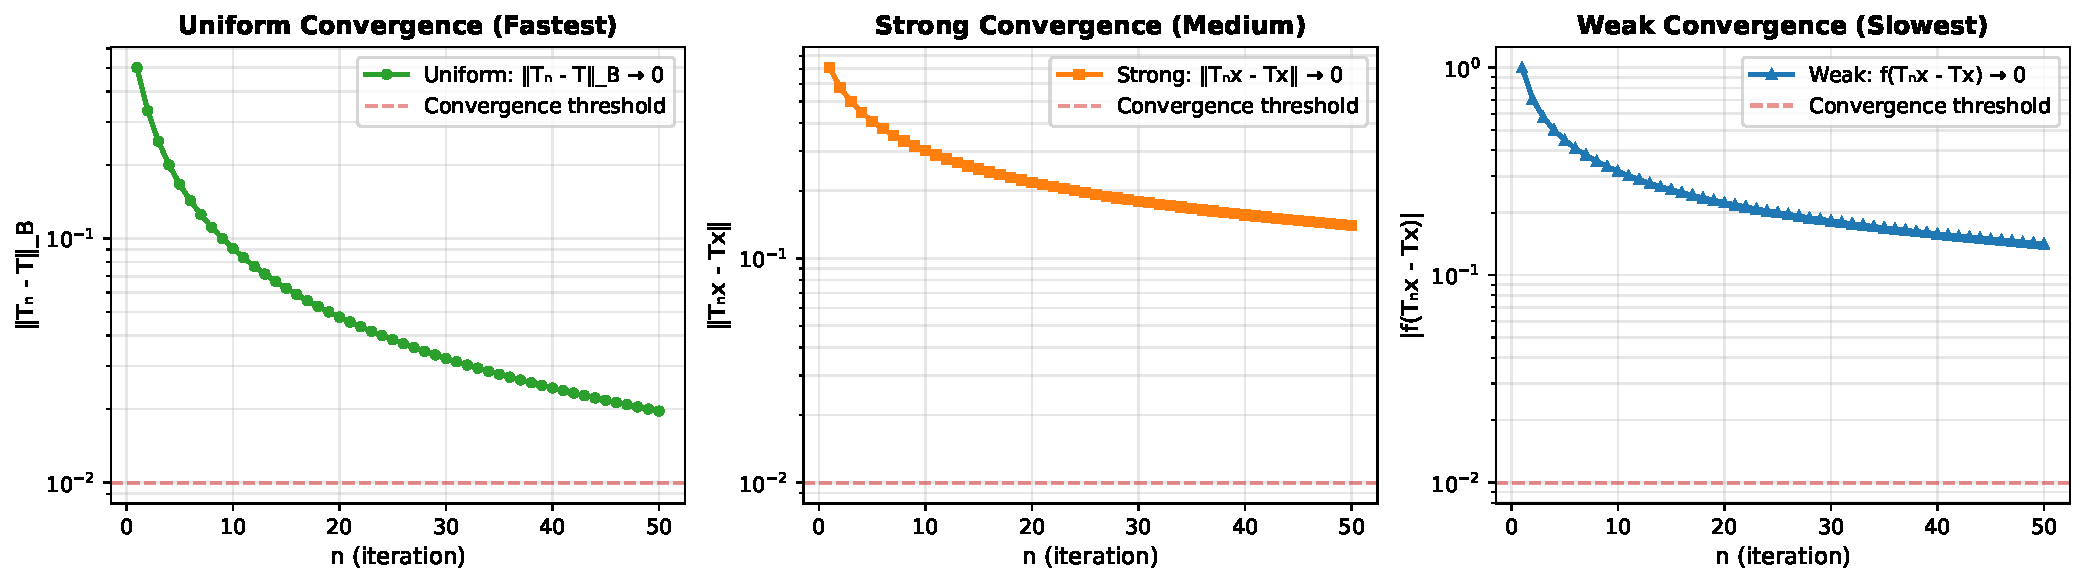
\includegraphics[width=\textwidth]{convergence_types.pdf}
    \end{center}
\end{frame}

\section{Key Theorems and Applications}

\begin{frame}{Corollary: Weakly Bounded Sets are Bounded}
    \begin{corollary}[Corollary 1.1]
        Let $C$ be a nonempty subset of a Banach space $X$. For each $f \in X^*$, suppose $f(C) = \{(x,f) : x \in C\}$ is a bounded set in $\mathbb{R}$. Then $C$ is bounded.
    \end{corollary}

    \vspace{0.5cm}

    \begin{block}{Proof Idea}
        \begin{enumerate}
            \item For each $x \in C$, define $T_x(f) = (x, f)$
            \item Each $T_x$ is a bounded linear operator: $T_x \in B(X^*, \mathbb{R})$
            \item Boundedness of $f(C)$ means $\sup_{x \in C} |T_x(f)| < \infty$
            \item By Uniform Boundedness Principle: $\sup_{x \in C} \|T_x\| < \infty$
            \item This means $C$ is bounded
        \end{enumerate}
    \end{block}

    \vspace{0.3cm}

    \begin{alertblock}{Significance}
        This shows that weak boundedness (boundedness under all linear functionals) implies actual boundedness.
    \end{alertblock}
\end{frame}

\begin{frame}{Finite Dimensionality Simplification}
    \begin{theorem}
        In a finite-dimensional normed space $X$, \textbf{all linear operators} $A : X \to Y$ are:
        \begin{itemize}
            \item Continuous
            \item Bounded
            \item Have closed graph
        \end{itemize}
    \end{theorem}

    \vspace{0.5cm}

    \begin{block}{Why?}
        In finite dimensions:
        \begin{enumerate}
            \item All norms are equivalent
            \item All linear operators can be represented as matrices
            \item Matrices are continuous (polynomial function of entries)
            \item No pathological unbounded operators exist
        \end{enumerate}
    \end{block}

    \vspace{0.3cm}

    \begin{alertblock}{Contrast with Infinite Dimensions}
        In infinite-dimensional spaces (like function spaces), unbounded linear operators are common and important!
    \end{alertblock}
\end{frame}

\begin{frame}{Summary of Key Results}
    \begin{center}
        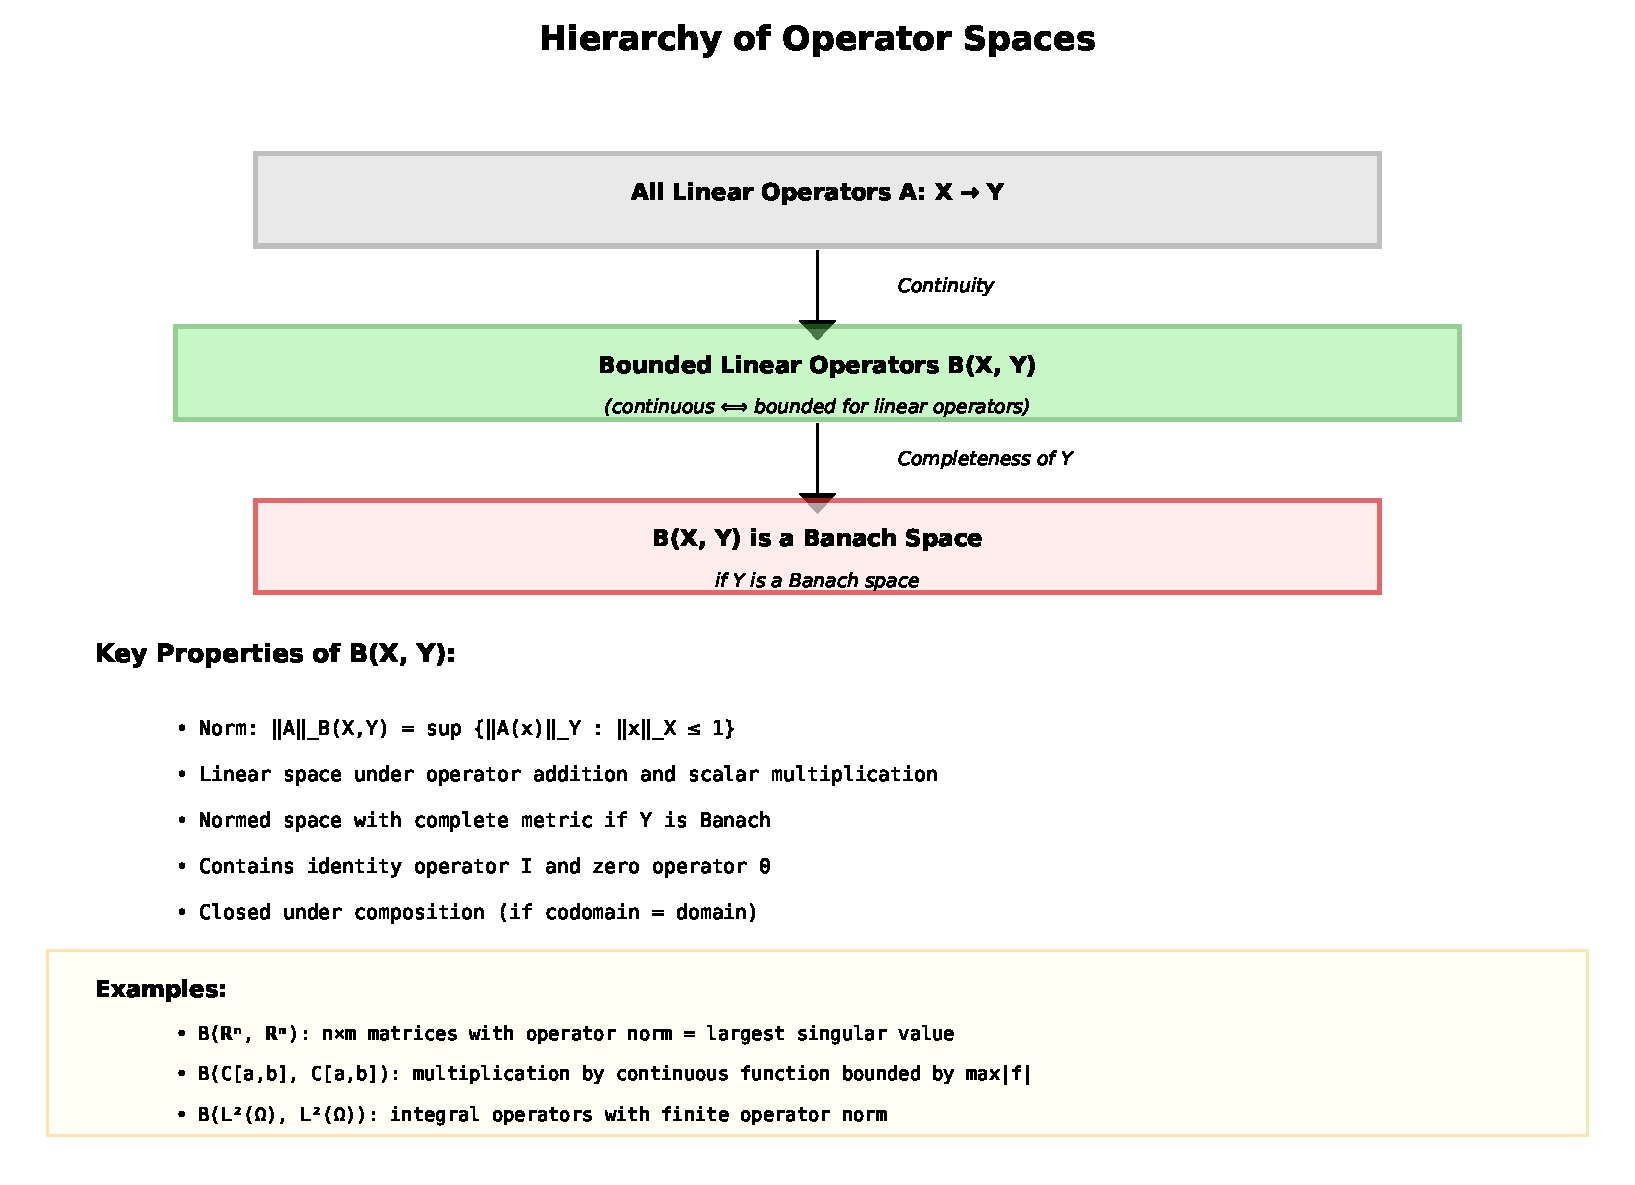
\includegraphics[width=\textwidth]{operator_spaces_hierarchy.pdf}
    \end{center}
\end{frame}

\section{Computational Examples}

\begin{frame}[fragile]{Example 1: Computing Operator Norm}
    \begin{block}{Problem}
        Let $A : \mathbb{R}^2 \to \mathbb{R}^2$ be the linear operator represented by matrix:
        $$A = \begin{pmatrix} 2 & 1 \\ 0 & 1 \end{pmatrix}$$
        Compute $\|A\|_B$ using the Euclidean norm.
    \end{block}

    \vspace{0.3cm}

    \begin{solution}
        The operator norm is the largest singular value of $A$:
        \begin{enumerate}
            \item Compute $A^T A = \begin{pmatrix} 4 & 2 \\ 2 & 2 \end{pmatrix}$
            \item Find eigenvalues: $\det(A^T A - \lambda I) = 0$
            \item $(4-\lambda)(2-\lambda) - 4 = \lambda^2 - 6\lambda + 4 = 0$
            \item $\lambda = 3 \pm \sqrt{5}$
            \item Largest eigenvalue: $\lambda_{\max} = 3 + \sqrt{5} \approx 5.236$
            \item Therefore: $\|A\|_B = \sqrt{3 + \sqrt{5}} \approx 2.288$
        \end{enumerate}
    \end{solution}
\end{frame}

\begin{frame}[fragile]{Example 2: Integral Operator on $L^2[0,1]$}
    \begin{block}{Problem}
        Let $X = L^2[0,1]$ and define $A : L^2[0,1] \to L^2[0,1]$ by:
        $$[Ax](t) = \int_0^1 K(t,s) x(s) \, ds$$
        where the kernel is $K(t,s) = ts$. Is $A$ bounded?
    \end{block}

    \vspace{0.3cm}

    \begin{solution}
        By Cauchy-Schwarz inequality:
        \begin{align*}
            |[Ax](t)|^2 &= \left|\int_0^1 ts \cdot x(s) \, ds\right|^2 \\
            &\leq \int_0^1 t^2 s^2 \, ds \cdot \int_0^1 x(s)^2 \, ds \\
            &= \frac{t^2}{3} \|x\|^2_{L^2}
        \end{align*}
        Integrating over $t$:
        \[\|Ax\|^2_{L^2} \leq \frac{1}{9} \|x\|^2_{L^2}\]
        Therefore $\|A\|_B \leq 1/3$ and \textbf{$A$ is bounded}.
    \end{solution}
\end{frame}

\begin{frame}[fragile]{Example 3: Checking Operator Continuity}
    \begin{lstlisting}
import numpy as np
from scipy import linalg

# Define linear operator as a matrix
def operator_norm(A, norm_type='spectral'):
    """
    Compute operator norm of matrix A
    norm_type: 'spectral' (singular value),
               'frobenius', '1', 'infinity'
    """
    return linalg.norm(A, ord=norm_type)

# Example: A = [[2, 1], [0, 1]]
A = np.array([[2., 1.], [0., 1.]])

# Compute different norms
print("Spectral norm (largest singular value):",
      operator_norm(A, 'spectral'))
print("Frobenius norm:", operator_norm(A, 'frobenius'))

# Verify boundedness: ||Ax|| <= ||A|| * ||x|| for all x
x = np.array([1., 1.])
Ax = A @ x
norm_Ax = linalg.norm(Ax)
norm_A = operator_norm(A)
norm_x = linalg.norm(x)

print(f"\n||Ax|| = {norm_Ax:.4f}")
print(f"||A|| * ||x|| = {norm_A * norm_x:.4f}")
print(f"Boundedness satisfied: {norm_Ax <= norm_A * norm_x}")
    \end{lstlisting}
\end{frame}

\begin{frame}{Key Definitions and Formulas}
    \begin{center}
        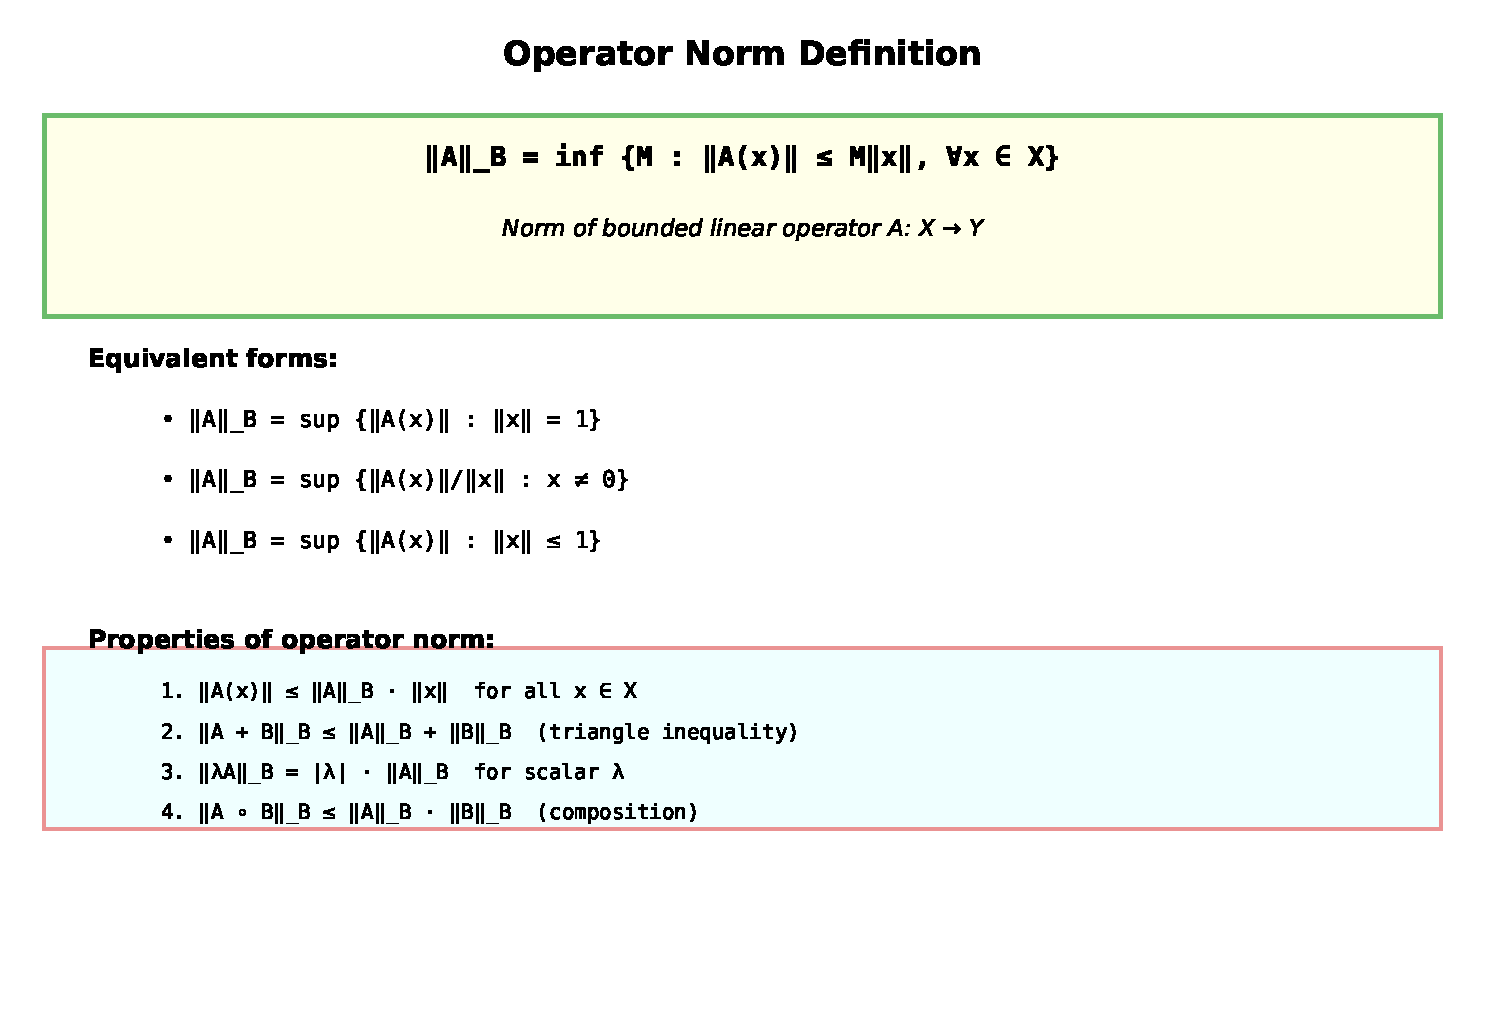
\includegraphics[width=\textwidth]{operator_norm_definition.pdf}
    \end{center}
\end{frame}

\begin{frame}{Visual Comparison: Linear vs Nonlinear}
    \begin{center}
        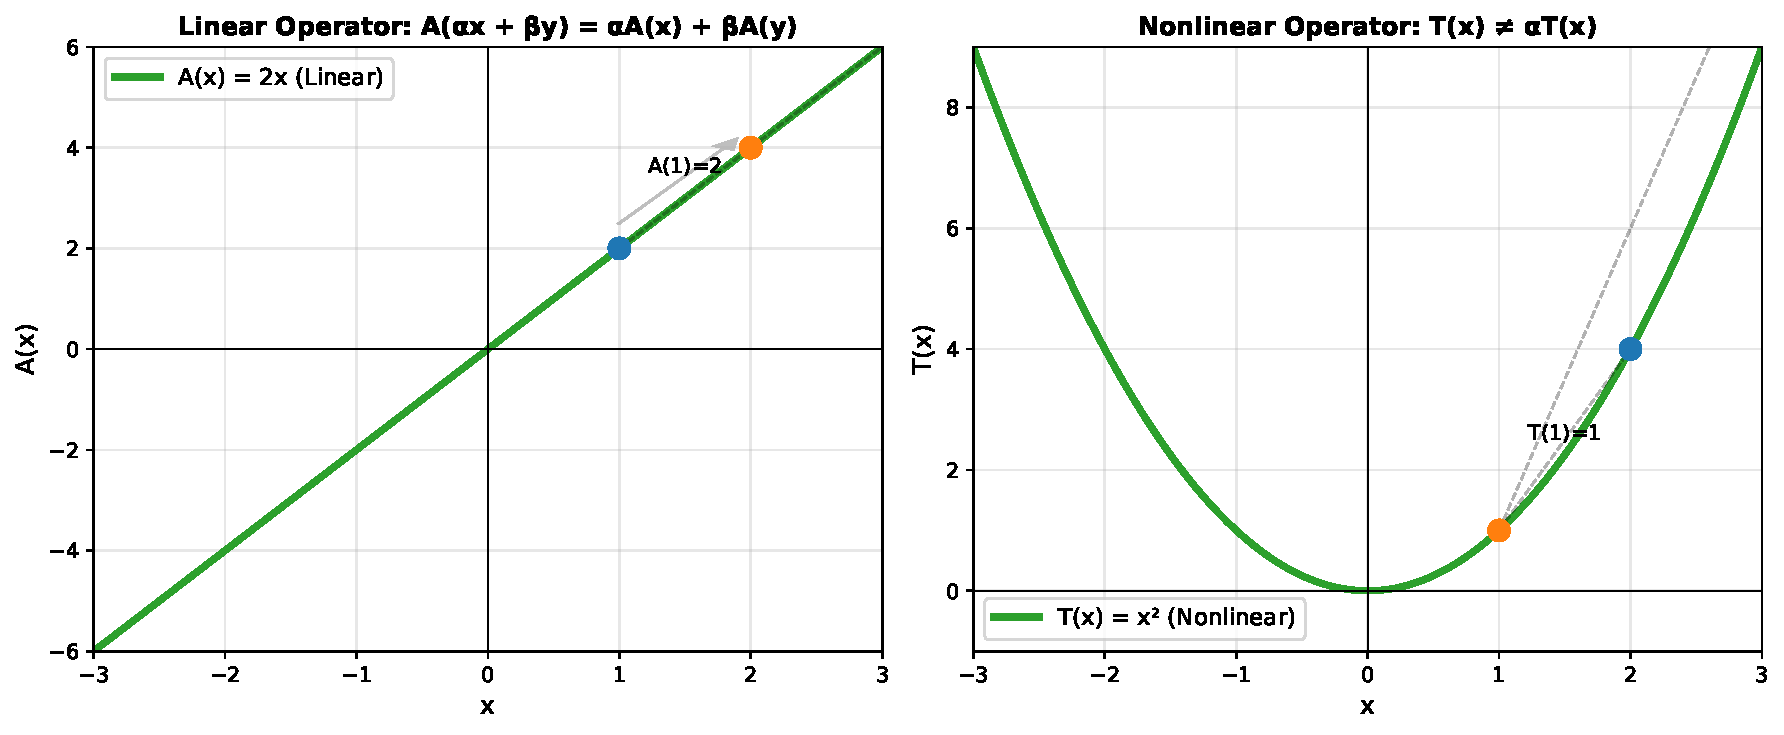
\includegraphics[width=\textwidth]{linear_vs_nonlinear.pdf}
    \end{center}
\end{frame}

\begin{frame}{Bounded vs Unbounded Operators}
    \begin{center}
        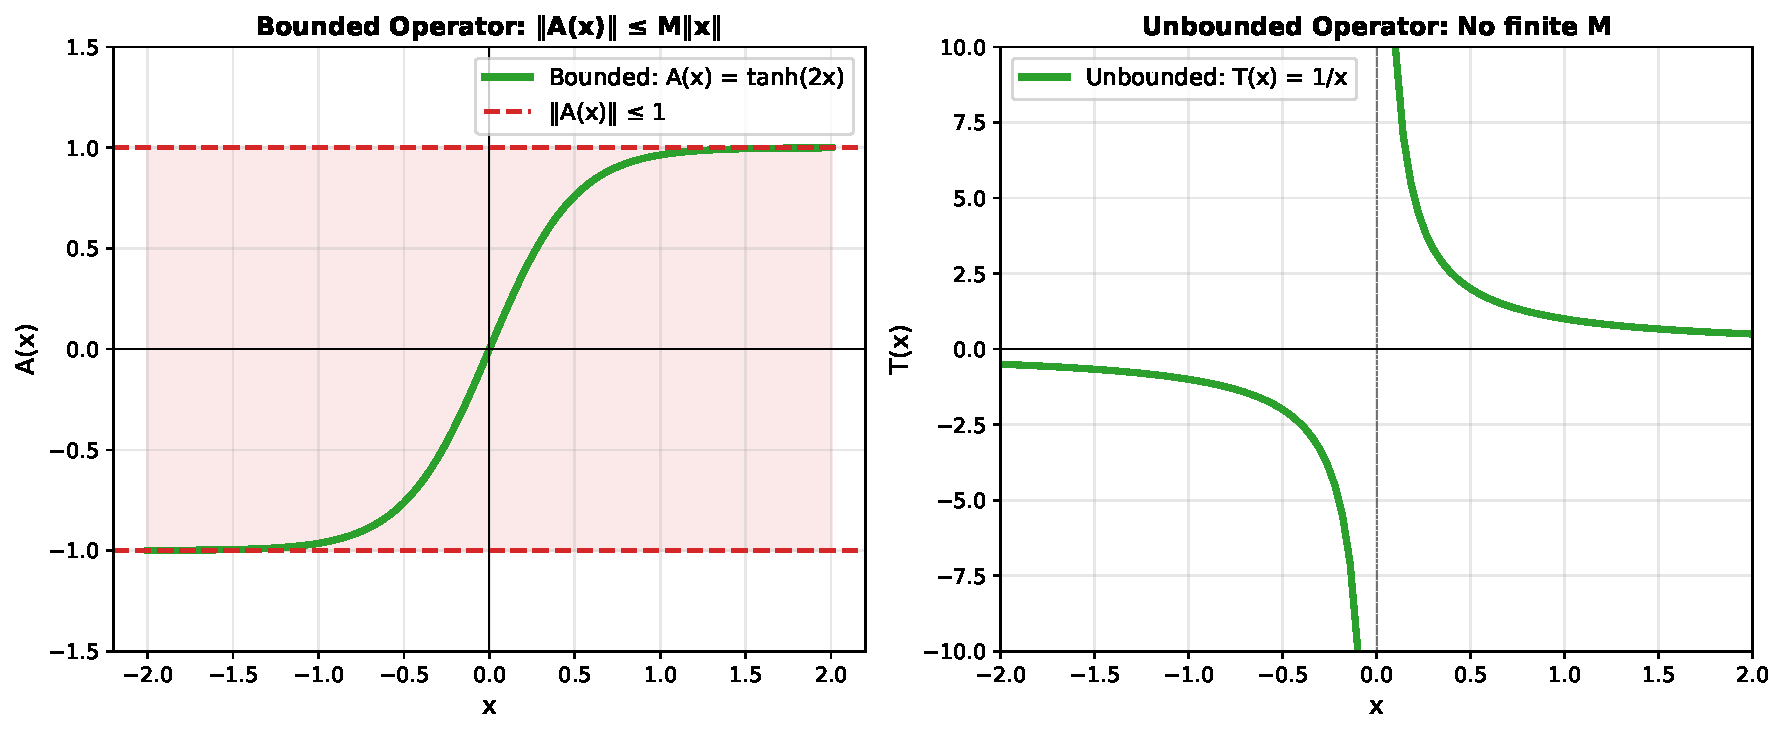
\includegraphics[width=\textwidth]{bounded_vs_unbounded.pdf}
    \end{center}
\end{frame}

\begin{frame}{The Continuity-Boundedness Connection}
    \begin{center}
        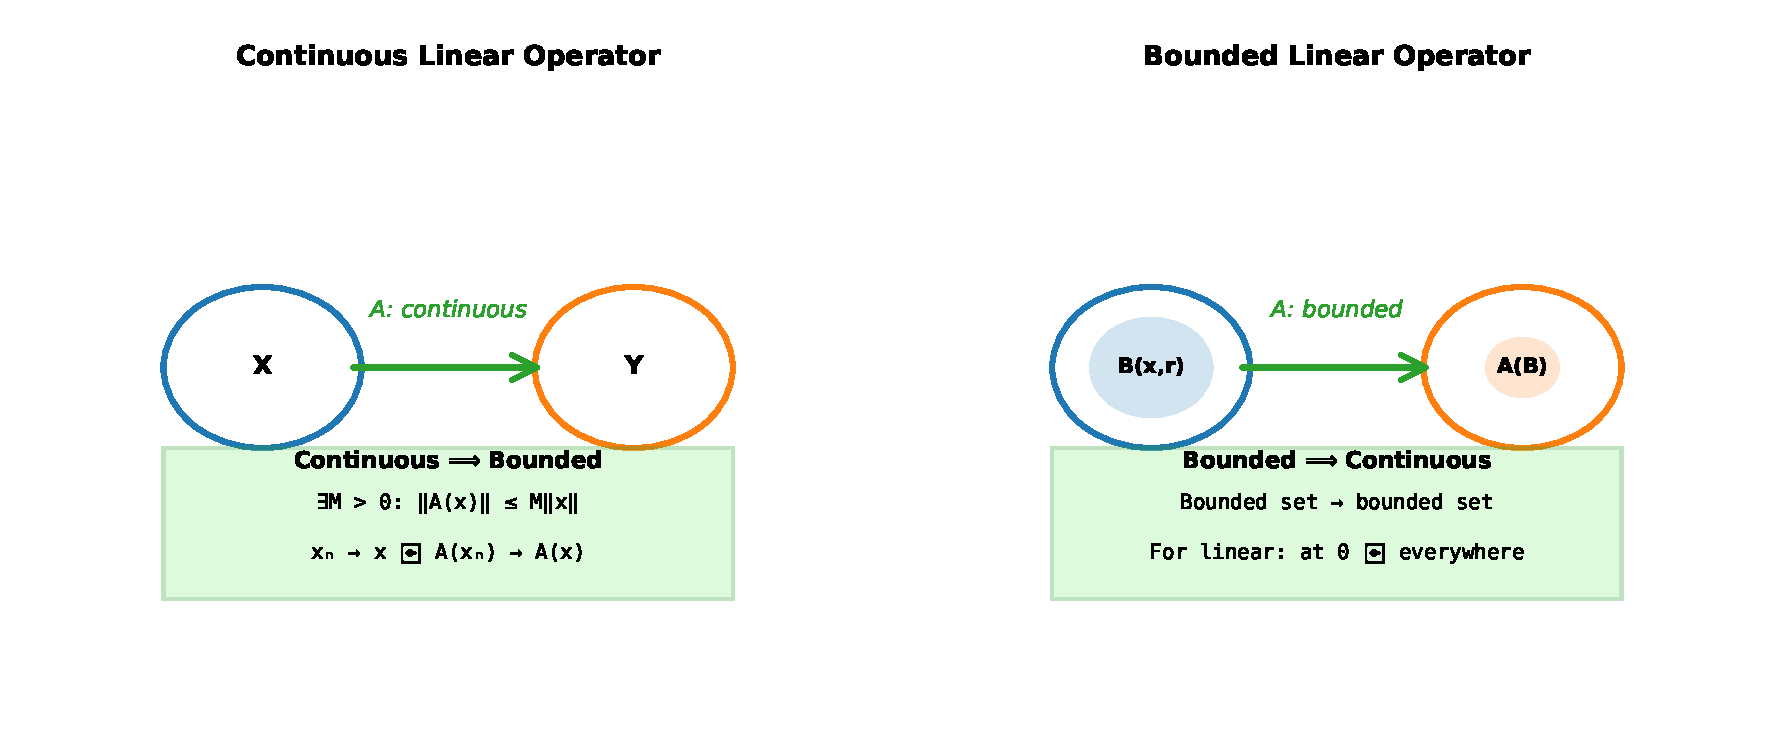
\includegraphics[width=0.95\textwidth]{continuity_boundedness_connection.pdf}
    \end{center}
\end{frame}

\section{Summary and Applications}

\begin{frame}{Main Takeaways}
    \begin{enumerate}
        \item \textbf{Linear operators} are the central objects in functional analysis, generalizing matrices to infinite-dimensional spaces

        \vspace{0.3cm}

        \item For linear operators: \textbf{boundedness} $\Leftrightarrow$ \textbf{continuity}

        \vspace{0.3cm}

        \item The \textbf{operator norm} $\|A\|_B$ uniquely determines boundedness and provides the standard for comparing operators

        \vspace{0.3cm}

        \item The space $B(X, Y)$ of bounded operators is itself a Banach space, enabling infinite-dimensional analysis

        \vspace{0.3cm}

        \item \textbf{Three types of convergence} exist: uniform (strongest), strong (medium), weak (weakest)

        \vspace{0.3cm}

        \item The \textbf{Uniform Boundedness Principle} connects pointwise and uniform boundedness—a corner stone result
    \end{enumerate}
\end{frame}

\begin{frame}{Applications in Analysis and PDEs}
    \begin{block}{Functional Analysis}
        \begin{itemize}
            \item Spectral theory: eigenvalues and eigenvectors of bounded operators
            \item Riesz representation theorem: correspondence between functionals and elements
            \item Lax-Milgram theorem: solvability of variational problems
        \end{itemize}
    \end{block}

    \begin{block}{Numerical Analysis}
        \begin{itemize}
            \item Iterative methods: convergence analysis via operator powers
            \item Finite element methods: approximation by bounded projection operators
            \item Error analysis: bounding errors using operator norms
        \end{itemize}
    \end{block}

    \begin{block}{PDEs and Physics}
        \begin{itemize}
            \item Differential operators: Laplacian, divergence, curl
            \item Integral equations: Fredholm and Volterra operators
            \item Quantum mechanics: observables as self-adjoint operators
        \end{itemize}
    \end{block}
\end{frame}

\begin{frame}{Further Reading and References}
    \begin{itemize}
        \item \textbf{Pathak (2018)}. An Introduction to Nonlinear Analysis and Fixed Point Theory. Springer.
        \begin{itemize}
            \item Chapter 1.3: Spaces of Bounded Linear Operators
            \item Chapter 1.3.1: Properties of Bounded Linear Operators
            \item Chapter 1.3.2: Convergence in $B(X,Y)$
        \end{itemize}

        \vspace{0.3cm}

        \item \textbf{Rudin (1991)}. Functional Analysis. McGraw-Hill.
        \begin{itemize}
            \item Comprehensive treatment of operator theory
            \item Spectral analysis and applications
        \end{itemize}

        \vspace{0.3cm}

        \item \textbf{Kreyszig (1978)}. Introductory Functional Analysis with Applications. Wiley.
        \begin{itemize}
            \item Intuitive exposition with applications
            \item Many worked examples and problems
        \end{itemize}
    \end{itemize}
\end{frame}

\begin{frame}[allowframebreaks]{References}
    \tiny
    \begin{thebibliography}{99}
        \bibitem{pathak2018} Pathak, H. K. (2018). \textit{An Introduction to Nonlinear Analysis and Fixed Point Theory}. Springer-Verlag.

        \bibitem{rudin1991} Rudin, W. (1991). \textit{Functional Analysis} (2nd ed.). McGraw-Hill International.

        \bibitem{kreyszig1978} Kreyszig, E. (1978). \textit{Introductory Functional Analysis with Applications}. John Wiley \& Sons.

        \bibitem{conway1990} Conway, J. B. (1990). \textit{A Course in Functional Analysis} (2nd ed.). Springer-Verlag.

        \bibitem{yosida1995} Yosida, K. (1995). \textit{Functional Analysis} (6th ed.). Springer-Verlag.

        \bibitem{brezis2010} Brezis, H. (2010). \textit{Functional Analysis, Sobolev Spaces and Partial Differential Equations}. Springer.
    \end{thebibliography}
\end{frame}

\begin{frame}{Conclusion}
    \begin{center}
        {\Large \textbf{Linear Operators: The Bridge Between} \\ \textbf{Linear Algebra and Functional Analysis}}

        \vspace{1cm}

        \begin{block}{Key Insight}
            Bounded linear operators provide a natural and powerful framework for generalizing matrix theory to infinite dimensions, with profound applications throughout mathematics, physics, and engineering.
        \end{block}

        \vspace{1cm}

        {\small Questions? Discussion?}
    \end{center}
\end{frame}

\end{document}
